\documentclass[11pt]{article}

% ============ PAQUETES ============
\usepackage[utf8]{inputenc}
\usepackage[T1]{fontenc}
\usepackage[margin=2.2cm]{geometry}
\usepackage{graphicx}
\usepackage{booktabs}
\usepackage{longtable}
\usepackage{array}
\usepackage{xcolor}
\usepackage{hyperref}
\usepackage{enumitem}
\usepackage{titlesec}
\usepackage{fancyhdr}
\usepackage{parskip}
\usepackage{ragged2e}
\usepackage{float}
\usepackage{caption}

% ============ COLORES ============
\definecolor{azulUTEQ}{HTML}{1F3864}
\definecolor{azulClaro}{HTML}{2E5395}
\definecolor{fondoTabla}{HTML}{F2F5FA}

% ============ FORMATO DE TÍTULOS ============
\titleformat{\section}{\Large\bfseries\color{azulUTEQ}}{\thesection}{1em}{}
\titleformat{\subsection}{\large\bfseries\color{azulClaro}}{\thesubsection}{1em}{}

% ============ ENCABEZADO/PIE DE PÁGINA ============
\pagestyle{fancy}
\fancyhf{}
\fancyhead[L]{\small Prueba Práctica -- Unidad IV -- Ingeniería de Requisitos (ISR-401)}
\fancyfoot[C]{\small\thepage}
\renewcommand{\headrulewidth}{0.4pt}

\hypersetup{
    colorlinks=true,
    linkcolor=azulClaro,
    urlcolor=azulClaro,
    citecolor=azulClaro,
    pdftitle={Prueba Practica Unidad IV - Solucion},
}

\renewcommand{\figurename}{Figura}
\begin{document}

% ======================================================================
% CARÁTULA
% ======================================================================
\begin{titlepage}
\centering
\vspace*{0.6cm}

{\large UNIVERSIDAD TÉCNICA ESTATAL DE QUEVEDO\par}
{\normalsize Facultad de Ciencias de la Ingeniería \textbullet{} Carrera de Ingeniería de Software\par}
\vspace{0.7cm}

{\Huge\bfseries\color{azulUTEQ} PRUEBA PRÁCTICA -- UNIDAD IV\par}
\vspace{0.3cm}
{\Large Validación, Gestión, Herramientas y Estándares de Requisitos\par}
\vspace{0.4cm}
{\large Ingeniería de Requisitos (ISR-401)\par}
{\large Docente: Ing. Gleiston Guerrero, Mg.\par}

\vspace{1cm}
\begin{tabular}{ll}
\textbf{Estudiante:} & Pérez Ruíz Carlos Andrés \\[0.4cm]
\textbf{Cédula / ID:} & 0955713136 \\[0.4cm]
\textbf{Fecha:} & Martes 11 de Agosto del 2026 \\[0.4cm]
\end{tabular}

\vspace{1cm}
{\bfseries URL del repositorio (Git):}\par
\vspace{0.3cm}
\url{https://github.com/cperezr3/IR_Evaluacion_Unidad_IV.git}

\vfill
{\small Documento de uso académico -- Ingeniería de Requisitos (ISR-401) -- UTEQ.\par}
\end{titlepage}

\section*{Resolución de la Evaluación}

\subsection*{P1. Modelo de datos - Diagrama de Clases UML}
Se modelan las cuatro clases del dominio con atributos tipados, identificadores subrayados, al menos una
operación por clase y las multiplicidades en los extremos de cada asociación.

\begin{figure}[h]
\centering
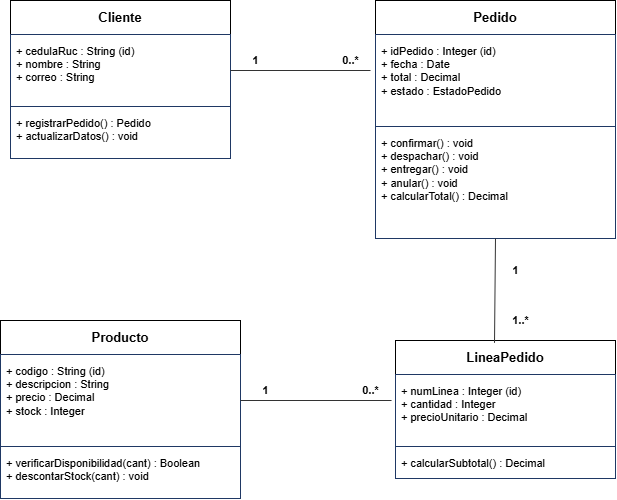
\includegraphics[width=\linewidth]{figures/p1_clases.png}
\caption{Diagrama de clases UML del dominio Sistema de Gestión de Pedidos.}
\end{figure}

\begin{itemize}[leftmargin=1.2cm]
  \item \textbf{Cliente (1) -- Pedido (0..*):} un cliente puede realizar cero o más pedidos; cada pedido
  pertenece a un único cliente.
  \item \textbf{Pedido (1) -- LíneaPedido (1..*):} cada pedido contiene una o más líneas; cada línea
  pertenece a un único pedido.
  \item \textbf{LíneaPedido (0..*) -- Producto (1):} cada línea referencia exactamente un producto; un
  producto puede aparecer en cero o más líneas de distintos pedidos.
\end{itemize}

\subsection*{P2. Modelo funcional - Diagrama de actividades UML}

\begin{figure}[H]
\centering
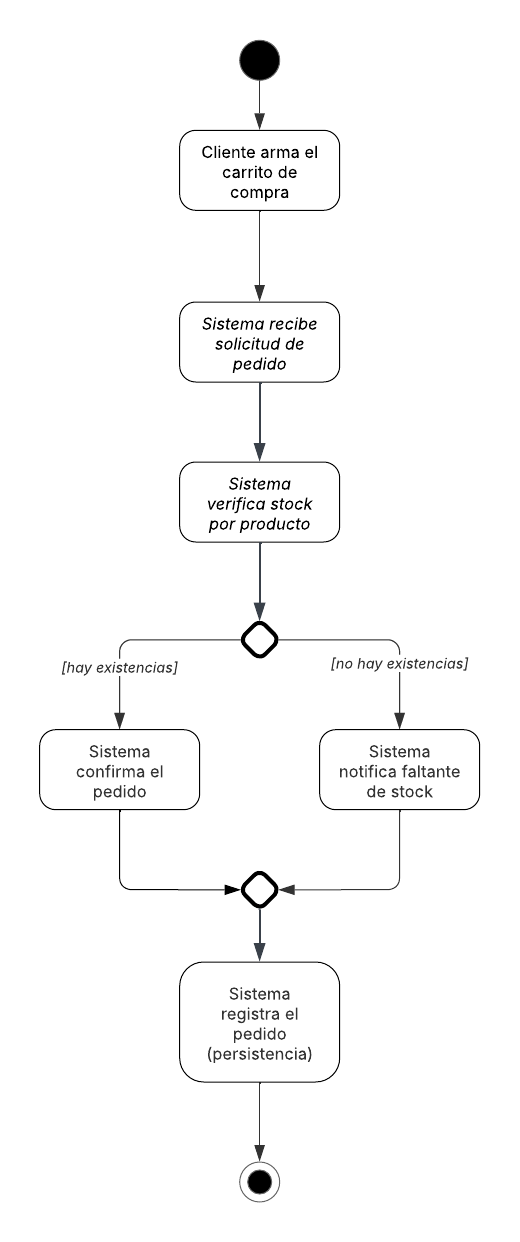
\includegraphics[width=0.55\linewidth]{figures/p2_actividades.png}
\caption{Diagrama de actividades UML del proceso ``Registrar pedido''.}
\end{figure}

\newpage

\subsection*{P3. Modelo de Comportamiento -- Máquina de estados UML}
Ciclo de vida del Pedido con los estados Registrado, Confirmado, Enviado (Despachado), Entregado y
Cancelado. Cada transición está etiquetada con su evento; la transición Registrado~$\rightarrow$~Confirmado
incluye la condición de guarda \textit{[stock disponible]}; Entregado es el estado final de aceptación. Se
factoriza la transición \textbf{anularPedido()} mediante el superestado \textbf{Activo}, que agrupa
Registrado, Confirmado y Enviado: desde cualquiera de esos tres estados el pedido puede anularse (guarda
\textit{[no entregado]}), evitando repetir la transición tres veces.

\begin{figure}[h]
\centering
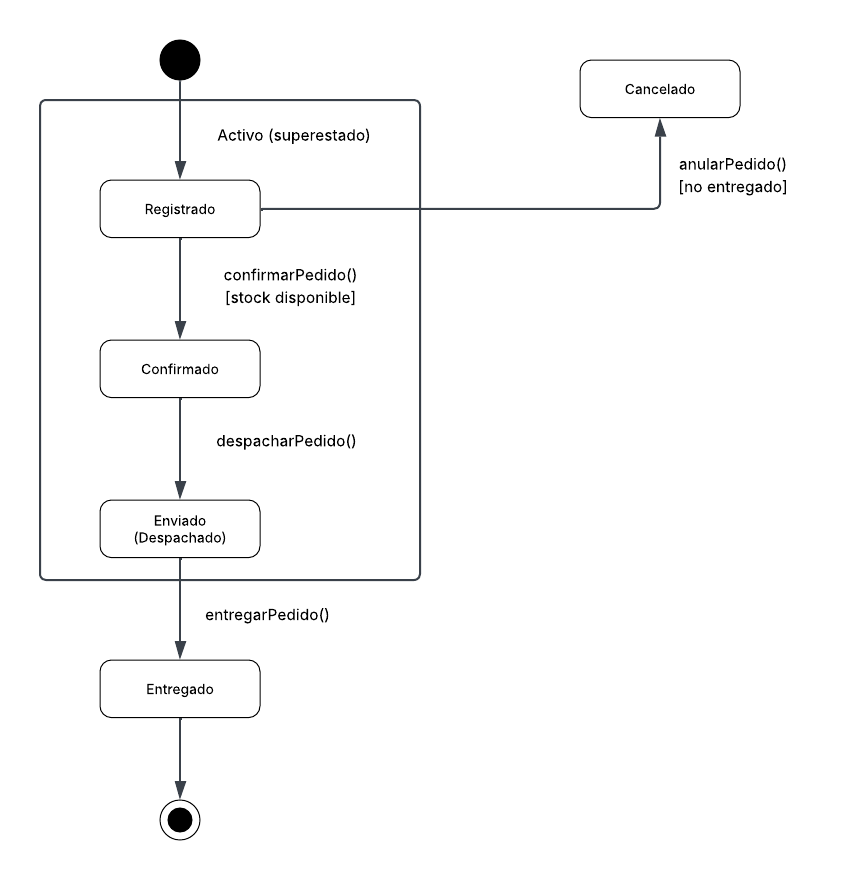
\includegraphics[width=0.6\linewidth]{figures/p3_estados.png}
\caption{Máquina de estados UML del ciclo de vida del Pedido.}
\end{figure}

\subsection*{P4. Consistencia entre las tres perspectivas}

\begin{longtable}{p{4.3cm}p{4.3cm}p{5.3cm}}
\caption{Tabla de verificación cruzada P3--P2--P1.}\\
\toprule
\textbf{Evento (P3)} & \textbf{Función/acción (P2)} & \textbf{Entidad/atributo modificado (P1)} \\
\midrule
\endfirsthead
\toprule
\textbf{Evento (P3)} & \textbf{Función/acción (P2)} & \textbf{Entidad/atributo modificado (P1)} \\
\midrule
\endhead
confirmarPedido() [stock disponible] & Sistema confirma el pedido & Pedido.estado $\rightarrow$
Confirmado \\
(sin evento explícito en P3) & Sistema notifica faltante de stock & --- (no persiste cambio de estado;
solo notificación) \\
despacharPedido() & (no modelada en P2 -- se ejecuta después del registro) & Pedido.estado
$\rightarrow$ Enviado \\
entregarPedido() & (no modelada en P2) & Pedido.estado $\rightarrow$ Entregado \\
anularPedido() [no entregado] & (no modelada en P2) & Pedido.estado $\rightarrow$ Cancelado \\
(evento implícito de registro) & Sistema registra el pedido (persistencia) & Pedido (nueva instancia) +
LíneaPedido (nuevas instancias) + Producto.stock (descuento) \\
\bottomrule
\end{longtable}

\textbf{Inconsistencia detectada:} el diagrama de actividades (P2) modela únicamente el subproceso
\textit{``Registrar pedido''} y termina en ``Sistema registra el pedido''; no incluye actividades para
\textbf{despachar}, \textbf{entregar} ni \textbf{anular} el pedido, aun cuando la máquina de estados (P3)
sí define esos tres eventos como transiciones válidas del ciclo de vida. Esto constituye una
inconsistencia de tipo \textbf{``evento sin función''}: existen eventos en el modelo de comportamiento que
no tienen una actividad correspondiente en el modelo funcional.

\textbf{Corrección aplicada:} se documenta que el diagrama de actividades P2 representa \textit{solo} el
subproceso de registro (alcance explícito del enunciado: ``Modele el proceso Registrar pedido''), y se
declara que los eventos despacharPedido(), entregarPedido() y anularPedido() deben modelarse como
\textbf{diagramas de actividad adicionales} (fuera del alcance de P2, pero exigidos por completitud del
dominio). Como corrección mínima dentro del alcance de P2, se añade una nota de extensión al nodo final
indicando que el pedido registrado continúa su ciclo de vida según la máquina de estados de P3, dejando
trazada explícitamente la relación entre ambos modelos.

\subsection*{P5. Especificación de requisitos con esquema de atributos}

\subsubsection*{RF-01 (Funcional)}
El sistema deberá verificar la disponibilidad de stock de cada producto de la línea de pedido al momento
de registrar un pedido, y deberá confirmar el pedido si existen existencias suficientes.

\begin{table}[h]
\centering
\begin{tabular}{ll}
\toprule
\textbf{Atributo} & \textbf{Valor} \\
\midrule
Identificador & RF-01 \\
Prioridad & Alta \\
Estado & Propuesto \\
Fuente & Enunciado del caso ``Sistema de Gestión de Pedidos'' \\
Estabilidad & Estable (no se prevén cambios frecuentes) \\
Versión & 1.0 \\
Método de verificación & Prueba funcional de caja negra \\
\bottomrule
\end{tabular}
\end{table}

\subsubsection*{RF-02 (Funcional)}
El sistema deberá permitir anular un pedido confirmado o despachado, siempre que no haya sido entregado,
actualizando su estado a Cancelado.

\begin{table}[h]
\centering
\begin{tabular}{ll}
\toprule
\textbf{Atributo} & \textbf{Valor} \\
\midrule
Identificador & RF-02 \\
Prioridad & Media \\
Estado & Propuesto \\
Fuente & Enunciado del caso ``Sistema de Gestión de Pedidos'' \\
Estabilidad & Estable \\
Versión & 1.0 \\
Método de verificación & Prueba funcional de caja negra \\
\bottomrule
\end{tabular}
\end{table}

\subsubsection*{RNF-01 (No funcional)}
El sistema deberá registrar un pedido en un tiempo menor a 3 segundos, medido desde el envío de la
solicitud hasta la confirmación en pantalla.\\
\textbf{Característica ISO/IEC~25010:2023:} Eficiencia de desempeño (tiempo de respuesta) -- umbral:
$<$~3\,s.

\begin{table}[h]
\centering
\begin{tabular}{ll}
\toprule
\textbf{Atributo} & \textbf{Valor} \\
\midrule
Identificador & RNF-01 \\
Prioridad & Alta \\
Estado & Propuesto \\
Fuente & Enunciado del caso ``Sistema de Gestión de Pedidos'' \\
Estabilidad & Estable \\
Versión & 1.0 \\
Método de verificación & Prueba de medición / benchmarking y auditoría de configuración \\
\bottomrule
\end{tabular}
\end{table}

\subsubsection*{RNF-02 (No funcional)}
El sistema deberá proteger los datos personales del cliente (cédula/RUC, nombre, correo) cifrando su
almacenamiento y restringiendo su acceso solo a usuarios con rol autorizado.\\
\textbf{Característica ISO/IEC~25010:2023:} Seguridad (confidencialidad) -- umbral: 100\% de los campos
personales cifrados en reposo.

\begin{table}[h]
\centering
\begin{tabular}{ll}
\toprule
\textbf{Atributo} & \textbf{Valor} \\
\midrule
Identificador & RNF-02 \\
Prioridad & Media \\
Estado & Propuesto \\
Fuente & Enunciado del caso ``Sistema de Gestión de Pedidos'' \\
Estabilidad & Estable \\
Versión & 1.0 \\
Método de verificación & Prueba de medición / benchmarking y auditoría de configuración \\
\bottomrule
\end{tabular}
\end{table}

\newpage
\subsection*{P6. Priorización MoSCoW }

\begin{longtable}{p{1.8cm}p{2.2cm}p{10cm}}
\caption{Priorización MoSCoW de los requisitos P5.}\\
\toprule
\textbf{Requisito} & \textbf{Categoría} & \textbf{Justificación} \\
\midrule
\endfirsthead
\toprule
\textbf{Requisito} & \textbf{Categoría} & \textbf{Justificación} \\
\midrule
\endhead
RF-01 & \textbf{Must have} & Sin verificación de stock y confirmación, el sistema no cumple su propósito
mínimo de gestionar pedidos correctamente; es viable e imprescindible desde el primer incremento. \\
RF-02 & Should have & Aporta valor operativo importante (gestión del ciclo de vida completo), pero el
sistema puede operar en una primera versión con anulación gestionada manualmente por soporte. \\
RNF-01 & \textbf{Must have} & El tiempo de respuesta es crítico para la experiencia de compra en línea;
un registro lento afecta directamente la conversión de ventas y es técnicamente viable de cumplir. \\
RNF-02 & Should have & La protección de datos personales es muy relevante y legalmente deseable, pero
puede introducirse en una segunda iteración con controles de acceso básicos ya vigentes como mitigación
temporal. \\
\bottomrule
\end{longtable}

\subsection*{P7. Validación por inspección}

\subsubsection*{Paso 1 -- Identificación de defectos (sin corregir)}

\begin{longtable}{p{1.6cm}p{2.3cm}p{1.5cm}p{8.5cm}}
\caption{Defectos detectados por inspección.}\\
\toprule
\textbf{Requisito} & \textbf{Propiedad evaluada} & \textbf{¿Cumple?} & \textbf{Defecto detectado} \\
\midrule
\endfirsthead
\toprule
\textbf{Requisito} & \textbf{Propiedad evaluada} & \textbf{¿Cumple?} & \textbf{Defecto detectado} \\
\midrule
\endhead
RF-01 & Singular & No & Combina dos acciones en un solo enunciado (verificar stock Y confirmar pedido);
debería separarse en dos requisitos singulares. \\
RF-02 & No ambiguo & Parcial & ``Siempre que no haya sido entregado'' es correcto, pero no especifica qué
ocurre con el stock previamente descontado al anular (falta regla de reversión). \\
RNF-01 & Verificable & Parcial & No indica bajo qué condiciones de carga (usuarios concurrentes) se mide
el umbral de 3\,s, lo que dificulta una verificación reproducible. \\
RNF-02 & Completo & Parcial & No especifica el algoritmo o estándar de cifrado mínimo exigido, dejando
abierto el nivel de protección real. \\
\bottomrule
\end{longtable}

\subsubsection*{Paso 2 -- Retrabajo (requisitos corregidos)}
\begin{itemize}[leftmargin=1.2cm]
  \item \textbf{RF-01a:} El sistema deberá verificar la disponibilidad de stock de cada producto de la
  línea de pedido al momento de registrar un pedido.
  \item \textbf{RF-01b:} El sistema deberá confirmar el pedido cuando exista stock suficiente para todas
  sus líneas.
  \item \textbf{RF-02 (corregido):} El sistema deberá permitir anular un pedido confirmado o despachado,
  siempre que no haya sido entregado, actualizando su estado a Cancelado y restituyendo automáticamente el
  stock previamente descontado de cada producto de sus líneas.
  \item \textbf{RNF-01 (corregido):} El sistema deberá registrar un pedido en un tiempo menor a 3
  segundos, medido en el percentil 95 bajo una carga de hasta 100 usuarios concurrentes, desde el envío de
  la solicitud hasta la confirmación en pantalla.
  \item \textbf{RNF-02 (corregido):} El sistema deberá proteger los datos personales del cliente
  (cédula/RUC, nombre, correo) cifrándolos en reposo con AES-256 y restringiendo su acceso solo a usuarios
  con rol autorizado, conforme a control de acceso basado en roles (RBAC).
\end{itemize}

\newpage
\subsection*{P8 -- Pruebas de aceptación trazadas}

\begin{longtable}{p{1.3cm}p{2.1cm}p{3.4cm}p{3.8cm}p{1.6cm}}
\caption{Pruebas de aceptación trazadas a los requisitos de P5.}\\
\toprule
\textbf{Prueba} & \textbf{Tipo} & \textbf{Entradas} & \textbf{Criterio de éxito} & \textbf{Traza a} \\
\midrule
\endfirsthead
\toprule
\textbf{Prueba} & \textbf{Tipo} & \textbf{Entradas} & \textbf{Criterio de éxito} & \textbf{Traza a} \\
\midrule
\endhead
PA-01 & Funcional & Pedido con 2 líneas; producto A con stock=5 (cant.\ pedida=2), producto B con
stock=0 (cant.\ pedida=1) & El sistema confirma la línea de A y notifica el faltante de B, sin confirmar
el pedido completo & RF-01a / RF-01b \\
PA-02 & Funcional & Pedido en estado Confirmado, solicitud de anulación & El pedido cambia a estado
Cancelado y el stock del producto se restituye en la cantidad exacta de la línea & RF-02 \\
PA-03 & No funcional (desempeño) & 100 solicitudes de registro de pedido concurrentes & El percentil 95
del tiempo de registro es menor a 3 segundos & RNF-01 \\
PA-04 & No funcional (seguridad) / regresión & Usuario sin rol autorizado intenta consultar datos
personales de un cliente vía API & El sistema deniega el acceso (HTTP 403) y los datos permanecen
cifrados en la base de datos & RNF-02 \\
\bottomrule
\end{longtable}

\newpage
\section*{Evidencia de evaluación formativa / SGA}

\begin{figure}[h]
\centering
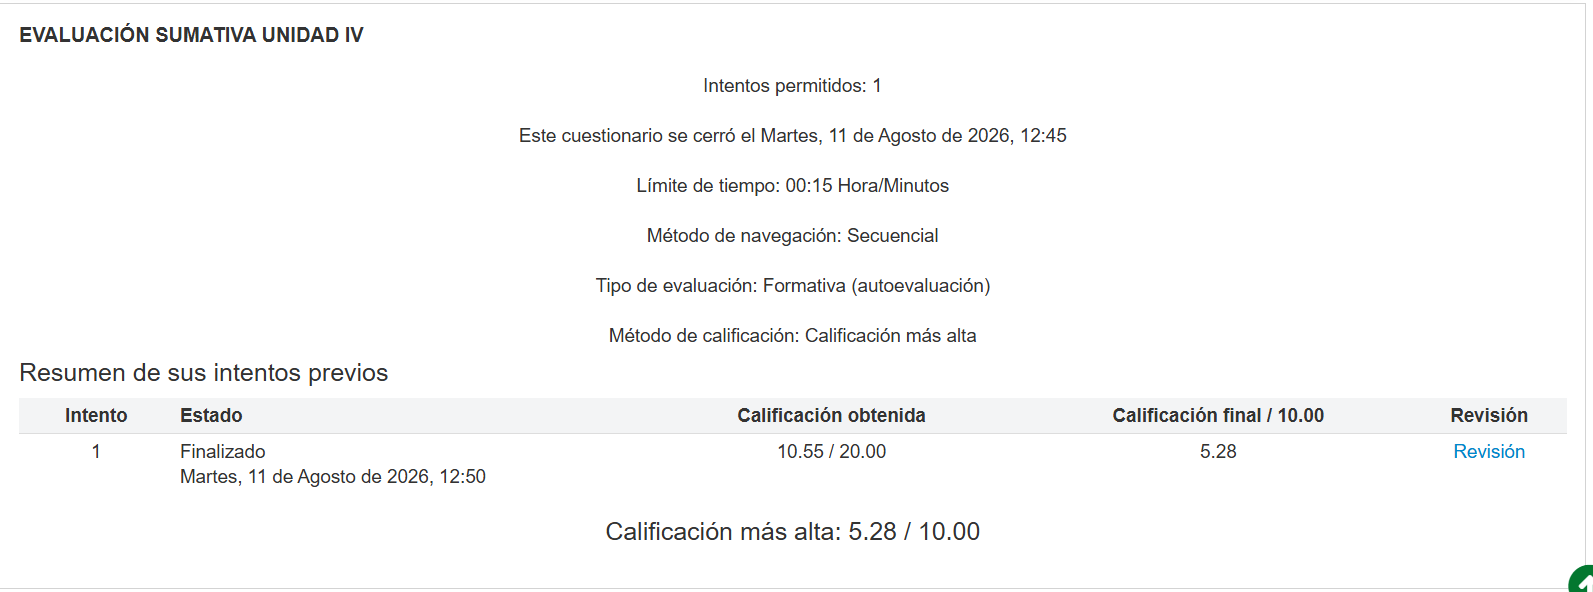
\includegraphics[width=0.9\linewidth]{figures/evaluacion_formativa.png}
\caption{Resultado de la evaluación formativa en el SGA. Calificación final: 5.28/10.00.}
\end{figure}

\begin{figure}[h]
\centering
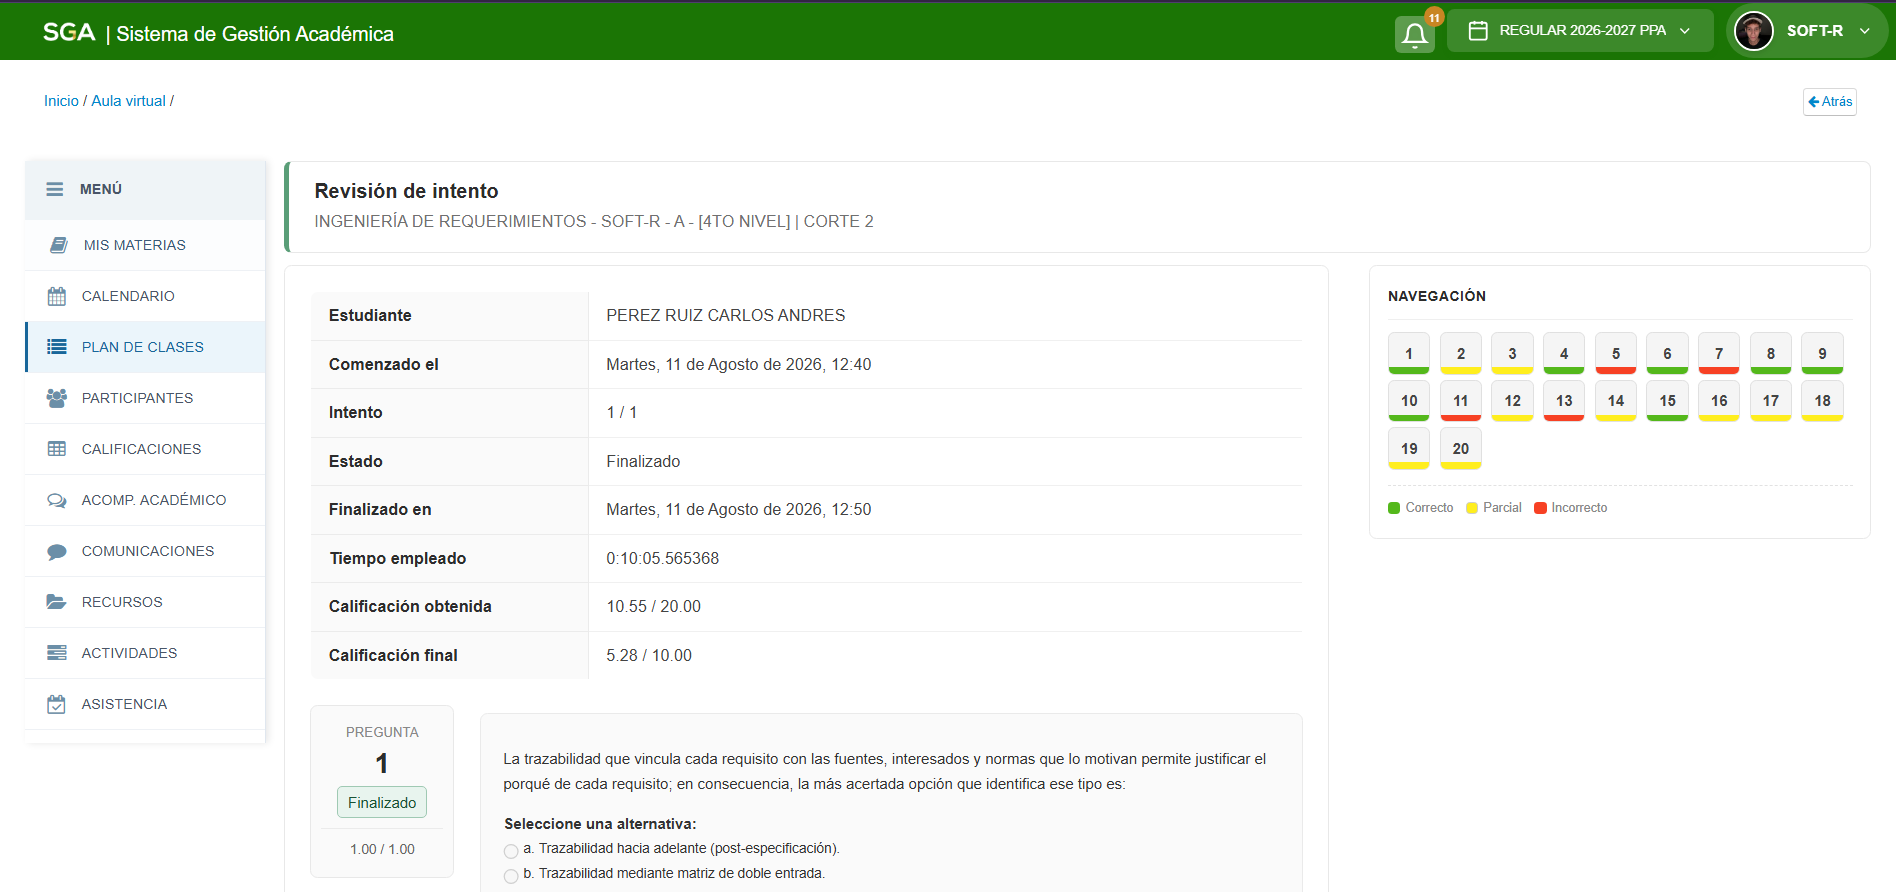
\includegraphics[width=0.9\linewidth]{figures/revision_intento.png}
\caption{Revisión del intento del cuestionario en el SGA (detalle de la evaluación rendida).}
\end{figure}

\end{document}
